\RequirePackage{luatex85}
\documentclass[tikz]{standalone}
\usepackage{mathtools, xcolor}

\newcounter{atom}

\newcommand\period[3]{
  \setcounter{atom}{#2}
  \foreach \n in {#3}{
    \addtocounter{atom}{-1}
    \draw({(\arabic{atom}-#2)*\x}, #1*-\x)
      node 
        [label=above:{\scalebox{5}{\arabic{atom}}}, outer sep=1mm]
        {\scalebox{10}{\smash\n\vphantom0}};
  }
}

\newcommand\I{\color{red!65!black}} % La's
\newcommand\J{\color{red!70!orange}} % Ac's
\newcommand\G{\color{orange}} % Transition metal
\newcommand\F{\color{yellow!55!black}} % Metal
\newcommand\E{\color{green!80!black!70!yellow}} % Metalloid
\newcommand\B{\color{green!50!blue}} % Nonmetal
\newcommand\A{\color{blue!80!white}} % Nobles
\newcommand\C{\color{blue!50!red}} % Group 1
\newcommand\D{\color{blue!20!red}} % Group 2
\newcommand\K{\color{gray}} % Unknown

\begin{document}
\ttfamily
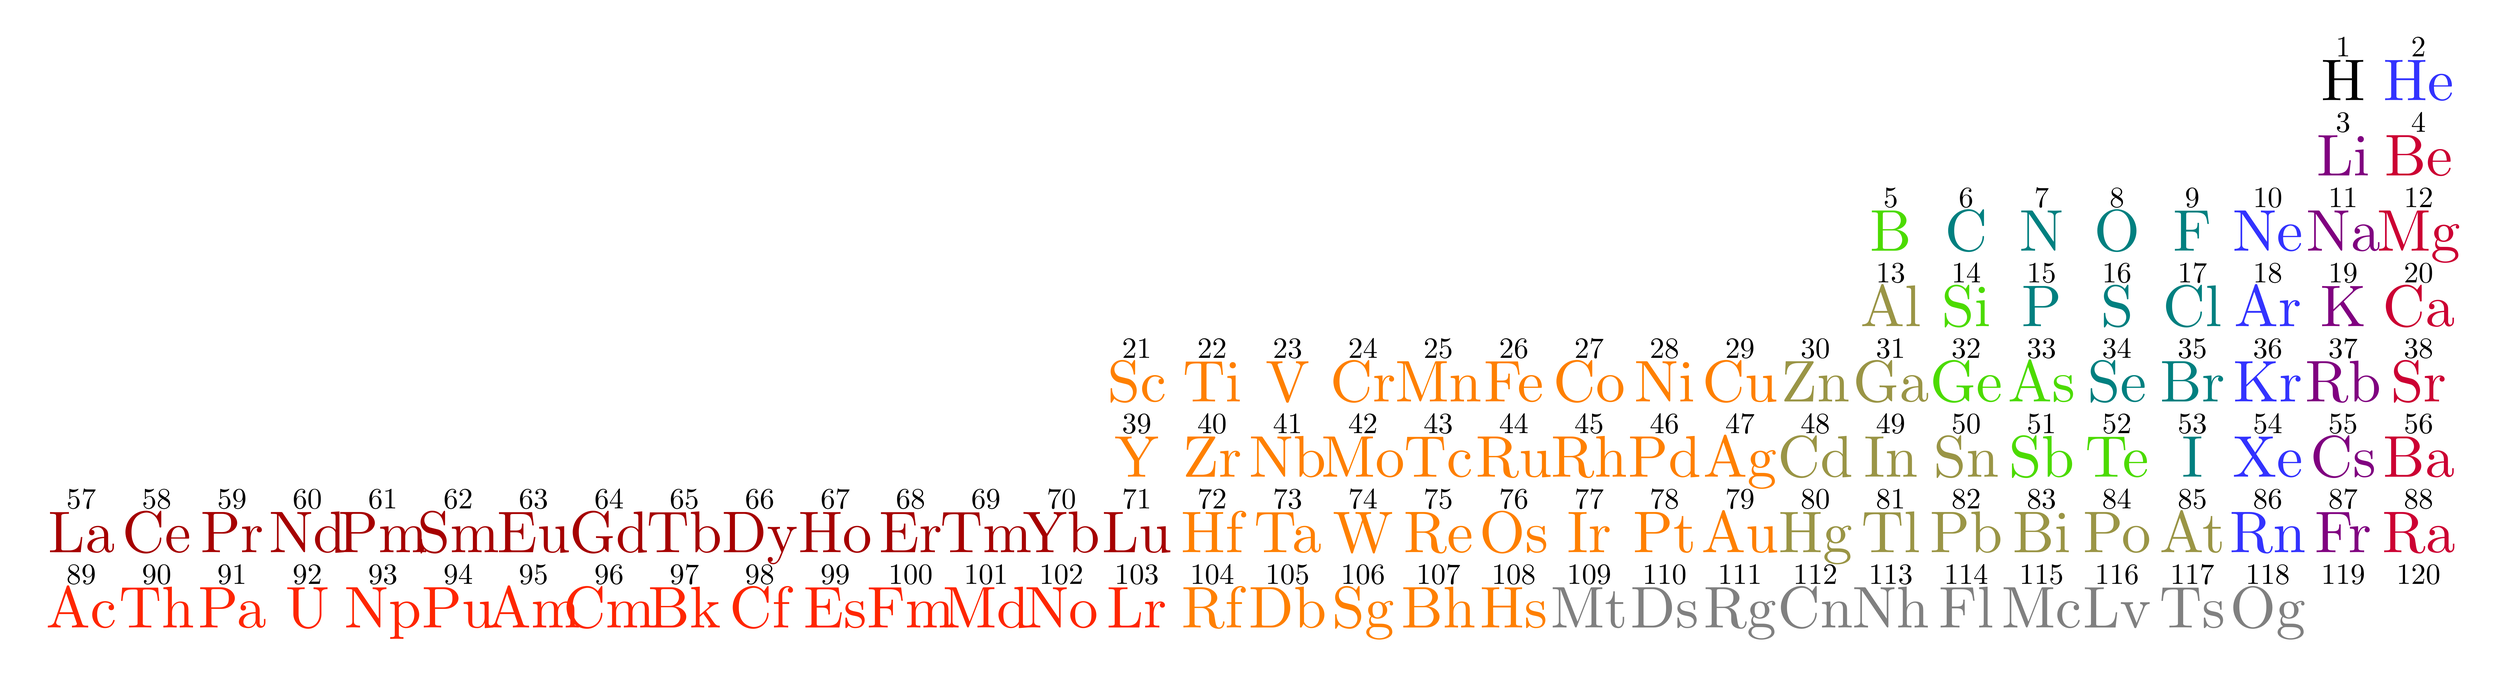
\begin{tikzpicture}
  \newcommand\x{45mm}
  \clip (0*\x, 1*\x) rectangle (-33*\x, -8*\x);
  \period0{3}{\A He, H}
  \period1{5}{\D Be, \C Li}
  \period2{13}{\D Mg, \C Na, \A Ne, \B F, \B O, \B N, \B C, \E B}
  \period3{21}{\D Ca, \C K, \A Ar, \B Cl, \B S, \B P, \E Si, \F Al}
  \period4{39}{\D Sr, \C Rb, \A Kr, \B Br, \B Se, \E As, \E Ge, \F Ga, \F Zn,\G Cu, \G Ni, \G Co, \G Fe, \G Mn, \G Cr, \G V, \G Ti, \G Sc}
  \period5{57}{\D Ba, \C Cs, \A Xe, \B I, \E Te, \E Sb, \F Sn, \F In, \F Cd, \G Ag, \G Pd, \G Rh, \G Ru, \G Tc, \G Mo, \G Nb, \G Zr, \G Y}
  \period6{89}{\D Ra, \C Fr, \A Rn, \F At, \F Po, \F Bi, \F Pb, \F Tl, \F Hg, \G Au, \G Pt, \G Ir, \G Os, \G Re, \G W, \G Ta, \G Hf, \I Lu, \I Yb, \I Tm, \I Er, \I Ho, \I Dy, \I Tb, \I Gd, \I Eu,\I Sm, \I Pm, \I Nd, \I Pr, \I Ce, \I La}
  \period7{121}{{}, {}, \K Og, \K Ts, \K Lv, \K Mc, \K Fl, \K Nh, \K Cn, \K Rg, \K Ds, \K Mt, \G Hs, \G Bh, \G Sg, \G Db, \G Rf, \J Lr, \J No, \J Md, \J Fm, \J Es, \J Cf, \J Bk, \J Cm,\J Am, \J Pu, \J Np, \J U, \J Pa, \J Th, \J Ac}
\end{tikzpicture}
\end{document}